
\documentclass{beamer}
\usepackage{pgfpages}
\setbeamertemplate{bibliography item}{\insertbiblabel}

% UNCOMMENT FOR FINAL COMPILATION WITH SPEAKER NOTES

%\setbeameroption{show notes on second screen=right} % Both
%\setbeamertemplate{note page}{\pagecolor{yellow!5}\insertnote}\usepackage{palatino}


\usepackage{graphicx}
\graphicspath{{images/}}


\author{Sam Barrett, 1803086}
\title{{Applications of genetic algorithms on fully-autonomous road networks} \\ \texorpdfstring
        {
\includegraphics[scale=0.1]{uobcrest.jpg}}
    }
\institute{{University of Birmingham}}
\date{\today}

\begin{document}

\begin{frame}
\titlepage
\end{frame}


\section{My Topic}
\begin{frame}{My Topic}
    \note{

        \begin{itemize}
            \item I am choosing to focus on the applications of Genetic Algorithms on Theoretical Fully autonomous road networks, with a view to extend into the possible applications of quantum computers on the field in the future. 
            \item  I feel the advent of fully autonomous road networks is a logical next step in making roads safer and more efficient through the use of technology.
            \item Fully autonomous driving trials have been legal in parts of the states for years with the UK following soon.
            \item Most research and all currently implemented systems focus on semi-autonomous environments whereby self-driving vehicles and humans co-exist on shared roads. 
            \item I propose it is both safer, easier and more efficient to implement, fully autonomous road networks where humans are not able to operate their vehicles.
            \item In such a system, sensor data would be shared between all vehicles near instantaneously allowing for much faster and less-selfish route planning, leading to net decreases in travel time. 

        \end{itemize}
    }
    \framesubtitle{Applications of Genetic Algorithms on Fully Autonomous Road Networks}

    \begin{itemize}

        \item Semi-autonomous vehicles are becoming more prevalent 
        \item Roads are becoming more congested with a 78\% increase in motor traffic since 1993 \cite{HighwaysEnglandNetwork2015}
        \item Fully autonomous vehicle trials have been legal in parts of the US since 2015\cite{AutonomousVehiclesSelfDriving}, with the UK set to follow by next year (2021)\cite{unknownUKWantsFully2019}
        \item Much of the current research into autonomous vehicle routing focuses on environments where human drivers are still present
        \item By removing the human element and working on theoretical \textit{fully autonomous road networks} we can make many useful assumptions about the behaviour of other vehicles
        \item The solution to road congestion is not to build bigger roads, it is to optimise the traffic flows.
        \item Just 78.2\% of journeys on the UK Highway Agencies roads were \textit{on time} in the year ending June 2014 \cite{measures02079443095ReliabilityJourneysHighways}

    \end{itemize}
\end{frame}

\begin{frame}{My Topic II}

    \begin{itemize}
        \item Huge undertaking to overhaul the existing motorway network even with a relatively small network such as that of the UK
        \item Such a system would require a government mandate projecting decades into the future
            \begin{itemize}
                \item e.g. All vehicles produced by 2035 will need to adhere to a universal routing standard.
                \item All car manufacturers would need to have the ability to produce fully autonomous vehicles \& have a standard sensor array.
            \end{itemize}
        \item Other problems that would need to be addressed include:
            \begin{itemize}
                \item Integrating priority-based routing to allow for emergency services to have a higher preference when routing vehicles
            \end{itemize}
        \item From a technical perspective, there are many things that need to be implemented to make such a system possible. 
            \begin{itemize}
                \item The encoding of routes into a real-valued string of genes
                \item The decoding of a real-valued string of genes to a route which a vehicle can take
                \item The implementation of a function to determine the fitness of an individual route. 
            \end{itemize}
    \end{itemize}

\end{frame}

\section{Literature}
\begin{frame}[allowframebreaks]

    \note{

        \begin{itemize}
            \item As previously mentioned most current research into GA applications within the car industry has a very broad scope. 
            \item Designing possible solutions that would fit into the current road networks easily. 
            \item I am intending to focus on a much more aspirational system, specifically looking at theoretical autonomous Motorways. 
            \item This enables me to overhaul the current road layout which was designed to aid human drivers not the overall efficiency of the system.
        \end{itemize}
        I have chosen to focus on GAs as opposed to other possible AI veins for a few reasons. 
        \begin{itemize}
            \item One personal reason is that I find them particularly interesting. 
            \item One more concrete reason is that they have the very useful property of being both probabilistically optimal and probabilistically complete. Meaning that given infinite time they not only will find \textit{a} solution but they will find \textbf{the} optimal solution. 
            \item And finally they have seen relatively minimal research in the field of vehicle planning with the limelight being taken by technologies such as Deep Learning or Reinforcement Learning
        \end{itemize}


    }

    \frametitle{Literature Review}
    I am currently intending to pursue my research assuming the absence of classical speed lanes as described by Kala and Warwick in \cite{kalaMotionPlanningAutonomous2013}. 

    I have chosen to focus on the applications of Genetic Algorithms on the field for 3 reasons: 
    \begin{enumerate}
        \item It is a class of optimisation algorithms that I find particularly interesting

        \item GAs are \textit{probabilistically optimal and complete}, i.e given infinite time, they will always produce the global optimal solution if such a solution exists

        \item It is a class of algorithm that has seen relatively minimal research in my the specific sub-area 
    \end{enumerate}
\end{frame}

\begin{frame}{Literature Review II}

    \note{
        \begin{itemize}
            \item A many of the technologies being researched with regards to vehicular planning suffer from the same problem from my point of view, they are \textit{black box approaches} meaning given a model, it is very difficult, if not impossible, to reason about and predict the decisions it makes. Such systems could end up making decisions based on imperfections in the training set. Such issues will make these systems less dependable and make people less likely to put their faith in them.
            \item In a paper from 2013, Kala and Warwick proposed a method of representing roads as a set of boundary functions in Cartesian space. All points on the road are defined using these functions as a new basis, this seems to be a good approach as it eliminates the possibility of plotting routes outside of the road space.

    \item in a book by Kala published in 2016, 3 years after his initial paper on autonomous planning, he talks about the possibility of planning using GAs to optimise Bézier curves. Each curve is determined by $n$ control points allowing for complex motions to be abstracted to a single objective function.
        \end{itemize}



    }


    \begin{itemize}
        \item Other approaches involve \textit{black box approaches}, such as the use of Reinforcement and deep inverse reinforcement learning by You et al.\cite{youAdvancedPlanningAutonomous2019}
        \item The downside of such an approach is that it is very difficult to reason and predict the actions of the system with a high degree of certainty. The ability to assure safety of such a critical system is very important and so GAs offer a much more predictable result
        \item Kala and Warwick \cite{kalaMotionPlanningAutonomous2013} proposed a system of two coordinate systems to safely represent points on the road within Cartesian space.
        \item In a book by Kala \cite{kalaOnroadIntelligentVehicles2016} he proposes GAs optimise Bézier curves representing the movement arc of a vehicle
    \end{itemize}
\end{frame}

\begin{frame}

    \note{
    
        here you can see a possible implementation as described by Kala in his book. You can see the control points determine the shape of the curve and allow the individual to avoid obstacles between two graph nodes.

        Below you can see the formal definition for a Bezier curve with $n$ control points where $C_j$ is the $j$th control point

    }
    \begin{figure}[KalaBezier]
        \centering
        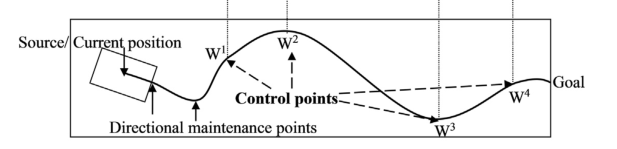
\includegraphics[width=0.8\linewidth]{kalaBezier.png}
        \caption{Bézier curves for route representation from Kala \cite{kalaOnroadIntelligentVehicles2016}}%
        \label{fig:.ext}
    \end{figure}

    \begin{itemize}
        \item A Bézier curve with $n$ control points is said to have a \textit{degree} of $n-1$ (initial point is called $P_0$ and is not counted in degree)
        \item A Bézier with a degree of 1 is a straight line between the two control points (the start and end point)
        \item Further control points \textit{bend} the line into a curve.
        \item The curve does not necessarily pass through all intermediate control points but it is determined by them.
        \item Bézier curves are smooth $\implies$ good for representing vehicle routes
    \end{itemize}
\end{frame}
\section{Methods}

\begin{frame}{Methods}
    \note{
        \begin{itemize}
            \item My project is more research focused rather than focused on producing a usable product.
            \item However, if a system such as the one I am proposing was ever implemented it would need to adhere to strict requirements to guarantee safety, performance and reliability
            \begin{itemize}
                \item It would need to be robust, by this I mean it would need to be well tested, written in a strongly typed language where it's actions can be reasoned about. A language such as Rust or OCaml have very strong compilers to the point where if they compile it is very rare for programs written in them to crash at runtime.
            \end{itemize}
        \end{itemize}

    }
    \begin{itemize}
        \item My Project is more researched based, will not yield a saleable \textit{product}
        \item If my proposed system were to be implemented, it would need to fit the following criteria
        \begin{itemize}
            \item Robust
            \item Secure
            \item Performant
            \item Run on relatively low-end hardware
            \item Written in a language with good support now and in the future 
            \item Able to compile to a binary to protect source code 
        \end{itemize}
    \end{itemize}
\end{frame}

\section{Bibliography}
\begin{frame}[allowframebreaks]
\frametitle{References}
\bibliographystyle{abbrv}
\bibliography{lib}
\end{frame}

\end{document}
